\chapter{Cloud Computing}
\label{sec:cc}
\section{Credentials}
StochSS provides the options to run jobs using the Amazon cloud infrastructures. In order to use Amazon Elastic Computing Cloud (EC2), Simple Storage Service (S3) and DynamoDB database, which are all required for running jobs in the cloud, you need an Amazon Web Services (AWS) account and a credential pair (consisting of a secret key and an access key) in hand. 

More information regarding how to create an AWS account and get credentials can be found here: \url{http://aws.amazon.com}

\subsection{Setting Credentials in StochSS}
You must set your credentials in StochSS manually (Figure \ref{fig:1}). Once StochSS validates these, you will be able to launch compute nodes and run jobs in the Amazon cloud.

\begin{figure}[!ht]
\centering
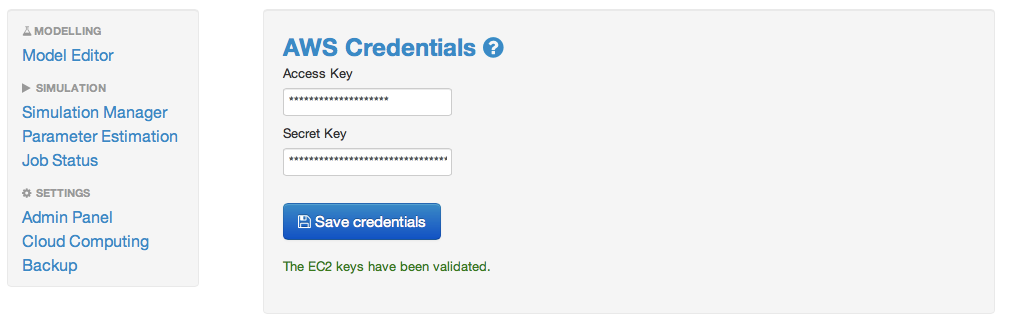
\includegraphics[scale=0.45]{T6/T6_fig_credentials.png}
\caption{Cloud Computing page - Credentials section}
\label{fig:1}
\end{figure}

\begin{enumerate}
\item Navigate to the main \textbf{Cloud Computing} page.
\item Copy your access key to the \textbf{Access Key} text box.
\item Copy your secret key to the \textbf{Secret Key} text box. 
\item Click \textbf{Save credentials} to validate and save your credentials.
\end{enumerate}

\subsection{Launching and Shutting Down Nodes}
Once valid credentials are entered, clicking \textbf{Launch nodes} (Figure \ref{fig:2}) by default will launch one c3.large Amazon instance. This first node is designated the \textbf{head node}. Any other nodes launched are called \textbf{worker nodes}. There can be zero or more worker nodes, and they are c3.larges instance types by default. For information on Amazon instance types, look here: \url{http://aws.amazon.com/ec2/instance-types/}. The head node must be a c3.large or c3.xlarge. The worker nodes can be any combination of t1.micro, m1.small, m3.medium, m3.large, c3.large, and c3.xlarge nodes (chosen in the \textbf{Advanced settings} menu).

Only one head node is needed to run jobs in the cloud. It is possible to access cloud data even when no head nodes are launched. Compute resources and storage resources are billed separately by Amazon. More details can be found at: \url{http://aws.amazon.com/ec2/pricing/}.

\begin{figure}[!ht]
\centering
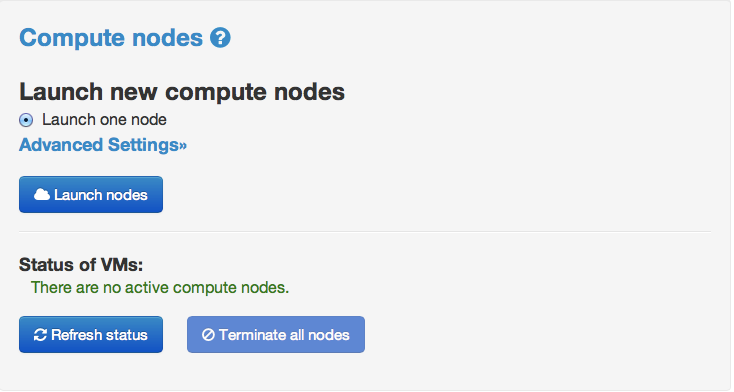
\includegraphics[scale=0.45]{T6/T6_fig_computenode1.png}
\caption{Cloud Computing page - Compute nodes default setting section}
\label{fig:2}
\end{figure}

Launching a node takes time. The \textbf{Refresh status} button can be used to check the launch progress. The \textbf{Terminate all nodes} button terminates all the nodes that StochSS started.

\section{Job Reproduction}
StochSS provides the flexibility to store simulation output in the cloud or delete it and regenerate it later. If simulations are fast but produce large amounts of data, reproducing data only when it is needed can save money.

\subsection{An Example on Job Reproduction}
Reproducing a cloud job is simple:

\begin{enumerate}
\item Launch a compute node.
\item Run a well-mixed or spatial model (everything except parameter estimation jobs can be reproduced).
\item Navigate to the \textbf{Job Status} page.
\item Click \textbf{view} beside the job you would like to reproduce.
\item Click \textbf{Delete Output} to delete output in the cloud. No reproduction action is available until you delete the output.
\item Once the output is deleted, the option to reproduce the job will be appear as shown in Figure \ref{fig:3}.
\item Choose a node type for reproduction. If there is no such instance type running, a warning will show up to guide you to the \textbf{Cloud Computing} page to launch one.
\item Click \textbf{Reproduce Results} to submit the reproduction request. This will automatically redirect to the \textbf{Job Status} page where the new job's status can be monitored.
\end{enumerate}

\begin{figure}[!ht]
\centering
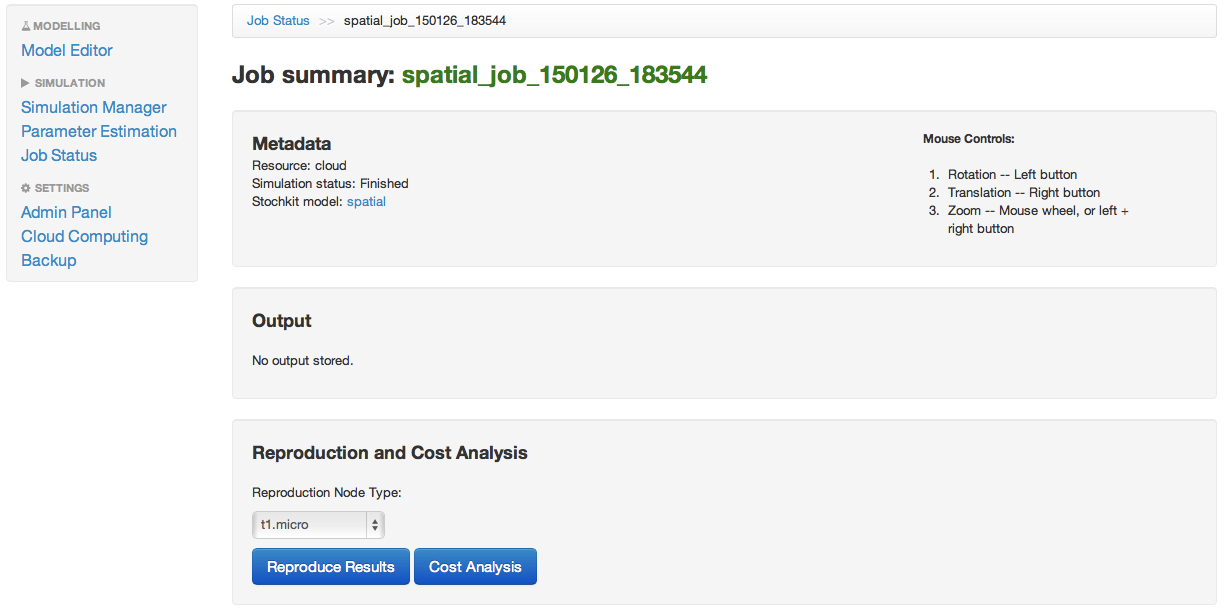
\includegraphics[scale=0.35]{T6/T6_fig_reproduction1.png}
\caption{Job summary page - reproduction available}
\label{fig:3}
\end{figure}

\section{Cost Analysis}
Because different instance types cost different amounts of money, it is not obvious which nodes are the cheapest for any given job type. StochSS allows manual measurement of job cost with the cost-analysis tool.

\subsection{An Example on Job Reproduction}

\begin{figure}[!ht]
\centering
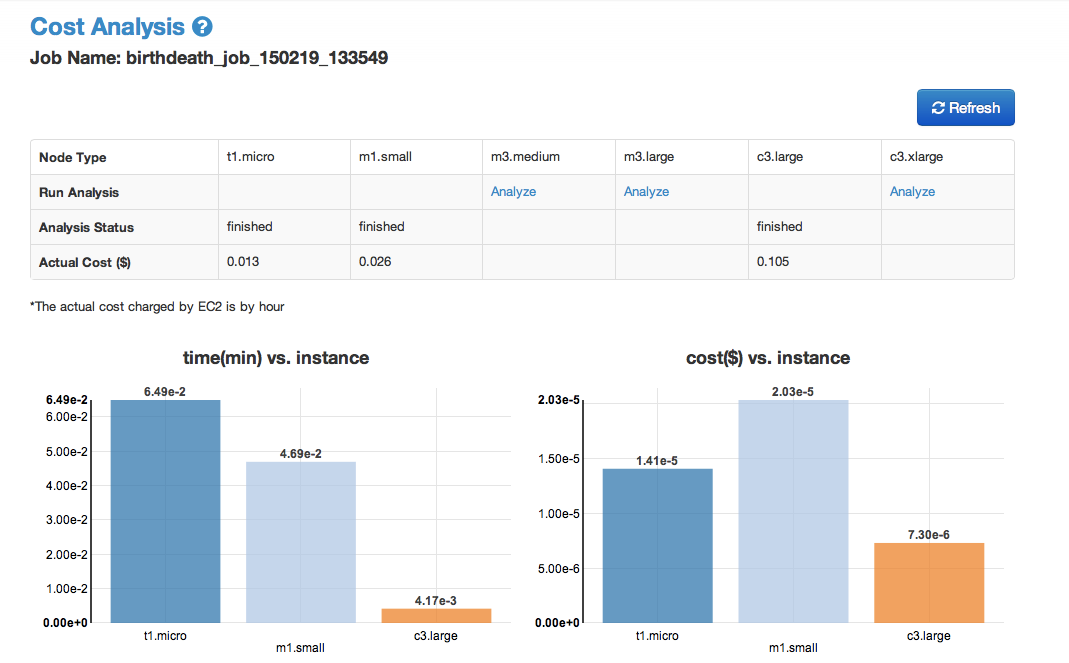
\includegraphics[scale=0.30]{T6/T6_fig_costanalysis.png}
\caption{Cost Analysis page}
\label{fig:cost-analysis}
\end{figure}

\begin{enumerate}
\item Run a well-mixed or spatial model.
\item Navigate to the \textbf{Job Status} page.
\item Click \textbf{view} beside the job you would like to analyze.
\item Click \textbf{Cost Analysis} in the \textbf{Reproduction and Cost Analysis} section.
\item By default, cost analysis should be available for whatever instance type the job was run on.
\item Click \textbf{Analyze} with any other node type you would like to run and analyze the job on. At least one node of this instance type must already be running.
\item The run times and costs of simulating the jobs are plotted on the screen as in Figure \ref{fig:cost-analysis}.
\end{enumerate}
